\documentclass[UTF8,a4paper,12pt,fontset=fandol]{ctexart}

% =========================
% Basic layout and packages
% =========================
\usepackage{geometry}
\usepackage{graphicx}
\usepackage{booktabs}
\usepackage{array}
\usepackage{tabularx}
\usepackage{longtable}
\usepackage{caption}
\usepackage{subcaption}
\usepackage{float}
\usepackage{xcolor}
\usepackage{enumitem}
\usepackage{fancyhdr}
\usepackage{hyperref}
\usepackage{amsmath}

\geometry{left=2.8cm,right=2.8cm,top=2.6cm,bottom=2.6cm}
\xeCJKsetup{CJKecglue={\hskip 0pt plus 0.08em\relax}}
\emergencystretch=2em
\linespread{1.35}
\setlength{\parindent}{2em}
\setlength{\parskip}{0.2em}
\setlist{nosep,leftmargin=2.4em}

% =========================
% Colors and link style
% =========================
\definecolor{SUFEBlue}{HTML}{1F4E79}
\definecolor{LightGray}{HTML}{F4F6F8}
\definecolor{MidGray}{HTML}{666666}

\hypersetup{
  colorlinks=true,
  linkcolor=SUFEBlue,
  urlcolor=SUFEBlue,
  citecolor=SUFEBlue,
  hypertexnames=false,
  pdfauthor={张思拓},
  pdftitle={基于大规模Steam游戏数据的市场结构、玩家反馈与平台生态变化分析}
}

% =========================
% Heading style
% =========================
\ctexset{
  section = {
    format = \heiti\zihao{3}\bfseries\color{SUFEBlue},
    beforeskip = 1.4em,
    afterskip = 0.8em
  },
  subsection = {
    format = \heiti\zihao{4}\bfseries,
    beforeskip = 1.0em,
    afterskip = 0.5em
  },
  subsubsection = {
    format = \heiti\zihao{-4}\bfseries,
    beforeskip = 0.8em,
    afterskip = 0.4em
  }
}

% =========================
% Header and footer
% =========================
\pagestyle{fancy}
\fancyhf{}
\fancyhead[L]{\small 《大数据处理技术》课程实践报告}
\fancyhead[R]{\small Ultimate\_Game\_Insights}
\fancyfoot[C]{\small \thepage}
\renewcommand{\headrulewidth}{0.4pt}
\renewcommand{\footrulewidth}{0pt}

% =========================
% Reusable placeholder box
% =========================
\newcommand{\placeholder}[1]{%
  \par\vspace{0.3em}
  \noindent\fcolorbox{gray!45}{LightGray}{%
    \begin{minipage}{0.94\linewidth}
      \small\color{MidGray}#1
    \end{minipage}
  }
  \par\vspace{0.7em}
}

\newcommand{\covertopic}[1]{%
  {\zihao{4}\begin{minipage}{12.2cm}\centering #1\end{minipage}\par}
  \vspace{0.95cm}
}

\newcommand{\coveritem}[2]{%
  {\zihao{3}#1：#2\par}
  \vspace{0.75cm}
}

% =========================
% Document metadata
% =========================
\newcommand{\reporttitle}{基于大规模Steam游戏数据的市场结构、玩家反馈与平台生态变化分析}
\newcommand{\studentname}{张思拓}
\newcommand{\studentid}{2025134009}
\newcommand{\projectname}{Ultimate\_Game\_Insights}

\begin{document}

% =========================
% Cover page
% =========================
\begin{titlepage}
  \thispagestyle{empty}
  \centering

  \vspace*{1.05cm}
  {\fontsize{32pt}{38pt}\selectfont\heiti 上海财经大学\par}

  \vspace{1.05cm}
  {\fontsize{26pt}{32pt}\selectfont\heiti 《大数据处理技术》课程实践报告\par}

  \vspace{3.0cm}
  \begin{center}
    \begin{minipage}{13.2cm}
      \centering
      \covertopic{\reporttitle}
      \coveritem{姓名}{\studentname}
      \coveritem{学号}{\studentid}
    \end{minipage}
  \end{center}

  \vfill
  {\zihao{4} \today\par}
\end{titlepage}

% =========================
% Abstract
% =========================
\pagenumbering{Roman}
\setcounter{page}{1}

\begin{center}
  {\heiti\zihao{3} 摘要}
\end{center}

\placeholder{在这里用 200--300 字概括报告内容。建议包括：数据来源、数据规模、使用的方法、核心分析方向、最重要的发现。请用你自己的话写核心观点。}

\noindent\textbf{关键词：} 大数据处理；Steam 游戏；市场结构；玩家反馈；标签分析；可视化分析

\newpage

% =========================
% Table of contents
% =========================
\tableofcontents
\newpage

\pagenumbering{arabic}
\setcounter{page}{1}

% =========================
% Main body
% =========================
\section{问题背景与研究目标}

\subsection{现实背景}
Steam是目前PC游戏领域中影响力较大的数字发行平台之一。平台上汇集了大量不同类型、不同规模和不同发行年代的游戏作品，既包括大型商业游戏，也包括独立游戏和中小团队作品。对于玩家来说，Steam不仅是购买和下载游戏的平台，也是查看游戏评价、浏览标签分类、了解游戏热度和参与社区互动的重要入口。

由于Steam长期积累了大量游戏信息和玩家反馈数据，其平台数据具有较强的分析价值。每款游戏通常包含发行时间、价格、支持平台、类型标签、开发商、发行商、玩家评论、推荐数、在线人数和游玩时长等字段。这些数据从不同角度记录了游戏的市场表现和玩家反馈，也为观察PC游戏市场的整体结构提供了较好的数据基础。

\subsection{研究问题}
基于Steam平台长期积累的游戏信息和玩家反馈数据，本次实践主要关注两个方面的问题。一方面，分析哪些Steam游戏更容易获得玩家关注。玩家关注度可以通过评论数量、推荐数、峰值在线人数和游玩时长等指标进行刻画，而价格、发行时间、平台支持情况、类型和标签等字段，则可以用于观察不同游戏特征与玩家关注度之间的关系。

另一方面，也关注Steam游戏市场在2024年5月到2025年3月之间的变化。通过对两个数据快照进行比较，可以观察这一阶段平台上的游戏数量、类型分布、标签结构、玩家反馈和热度表现是否出现变化。

\section{数据来源与字段说明}

\subsection{数据集来源}
本次实践使用的数据集为Kaggle平台上的\href{https://www.kaggle.com/datasets/artermiloff/steam-games-dataset/data}{Steam Games Dataset 2025}。该数据集通过Steam商店页面爬取整理得到，并结合Steam API和Steam Spy等数据来源，收集了Steam平台上大量游戏的相关信息。

数据集更新至2025年3月，包含原始解析版本和清洗版本两类文件。其中，清洗版本去除了重复游戏和playtest版本，更适合用于后续的统计分析。数据内容涵盖游戏基本信息、发行时间、价格、平台支持情况、玩家评论、热度指标、类型和标签等字段，能够较好地反映Steam平台游戏数据的整体情况。

\subsection{数据规模}
该数据集由4个CSV文件组成，原始文件总大小约为1.7GB，包含2024年5月和2025年3月两个时间快照。每个时间快照都提供了full版本和cleaned版本，其中full版本保留的信息更完整，cleaned版本则去除了重复游戏和playtest版本，更适合进行统计分析。

2025年3月cleaned版本约447MB，包含约89,619行数据；2024年5月cleaned版本约403MB，包含约83,647行数据。两个时间快照的存在，使得数据不仅可以用于观察Steam平台在2025年3月时的整体情况，也可以用于比较2024年到2025年之间游戏数量和平台生态的变化。

\begin{table}[H]
  \centering
  \caption{主要数据文件说明}
  \begin{tabularx}{0.95\textwidth}{lrrX}
    \toprule
    文件名 & 约文件大小 & 约行数 & 用途 \\
    \midrule
    games\_march2025\_cleaned.csv & 447MB & 89,619 & 主分析文件 \\
    games\_march2025\_full.csv & 450MB & 94,949 & 2025 完整字段文件 \\
    games\_may2024\_cleaned.csv & 403MB & 83,647 & 快照对比文件 \\
    games\_may2024\_full.csv & 405MB & 87,807 & 2024 完整字段文件 \\
    \bottomrule
  \end{tabularx}
\end{table}

\subsection{字段类型}
从字段结构来看，该数据集属于表格数据，其数据字段可以大致分为数值型、类别型、时间型、多标签型和文本型几类。其中，价格、评论数量、推荐数、峰值在线人数和游玩时长等字段属于数值型字段，可以用于统计和比较；平台支持情况、开发商、发行商等字段属于类别型字段，可以用于分组分析；发行日期属于时间型字段，可以用于观察游戏发行年份和市场变化趋势。

此外，数据集中还包含类型、分类和标签等多标签字段，这类字段往往不是单一取值，而是同时记录一款游戏的多个市场定位特征。游戏简介、详细描述等内容则属于文本型字段，能够补充说明游戏内容和主题。不同字段类型对应的分析方式并不相同，因此在后续处理前，需要先对字段结构进行识别和整理。

\section{大规模表格数据处理方法}

\subsection{读取风险与处理策略}
由于原始CSV文件体积较大，并且字段中包含较长的文本描述和多标签信息，如果每次分析都直接读取完整文件，会带来较高的读取时间和内存开销。尤其是在反复调试代码和生成图表时，重复加载全部字段不仅效率较低，也容易让后续分析过程变得不稳定。

因此，在实际处理时，不会把完整的表格反复作为直接分析对象，而是先根据分析目标选择需要使用的核心字段。例如，在市场结构分析中主要关注发行时间、价格、平台、类型和标签字段；在玩家反馈分析中则重点读取评论数量、好评率、推荐数、峰值在线人数和游玩时长等字段。通过减少无关字段和长文本字段的重复读取，可以降低数据读取压力，也让后续分析更加集中。

同时，对于后续多次使用的核心数据，采用中间数据形式进行保存，避免每个分析步骤都从原始数据重新开始。这样既保留了原始数据的完整性，也提高了后续清洗、特征工程和可视化分析的效率。

\subsection{工具对比}
为了判断在这种大规模表格数据中，不同工具更适合承担什么任务，本次实践对pandas、duckdb和polars进行了简单对比。主要选取了三个与后续分析直接相关的任务作为评价维度：一是选列读取，即只读取后续分析需要的核心字段；二是年度聚合，即根据发行日期统计不同年份的游戏数量和相关指标；三是Parquet转换与读取，即观察列式中间文件是否能提高后续重复分析的效率。

从测试结果来看，pandas的优势在于使用直观，适合进行常规数据检查、结果整理和图表展示，但在直接读取CSV和聚合时速度相对较慢；duckdb适合进行SQL式查询和分组聚合，在年度汇总这类任务中表达较清晰，内存变化也相对较小；polars在选列读取、聚合和Parquet读写中整体速度较快，更适合承担大表读取和批量转换任务。Parquet文件在只保留核心字段后，文件体积明显小于原始CSV，也更适合后续反复读取。

因此，后续处理采用将核心字段转为Parquet，分析阶段按任务选择工具的方案。将需要多次使用的字段经过筛选和清洗后保存为可再生成的Parquet文件；pandas主要用于结果检查和可视化，duckdb用于部分汇总查询，polars用于较高性能的数据读取和格式转换。这样既保留了原始数据的完整性，也减少了后续反复读取完整数据带来的时间和内存开销。

\begin{figure}[H]
  \centering
  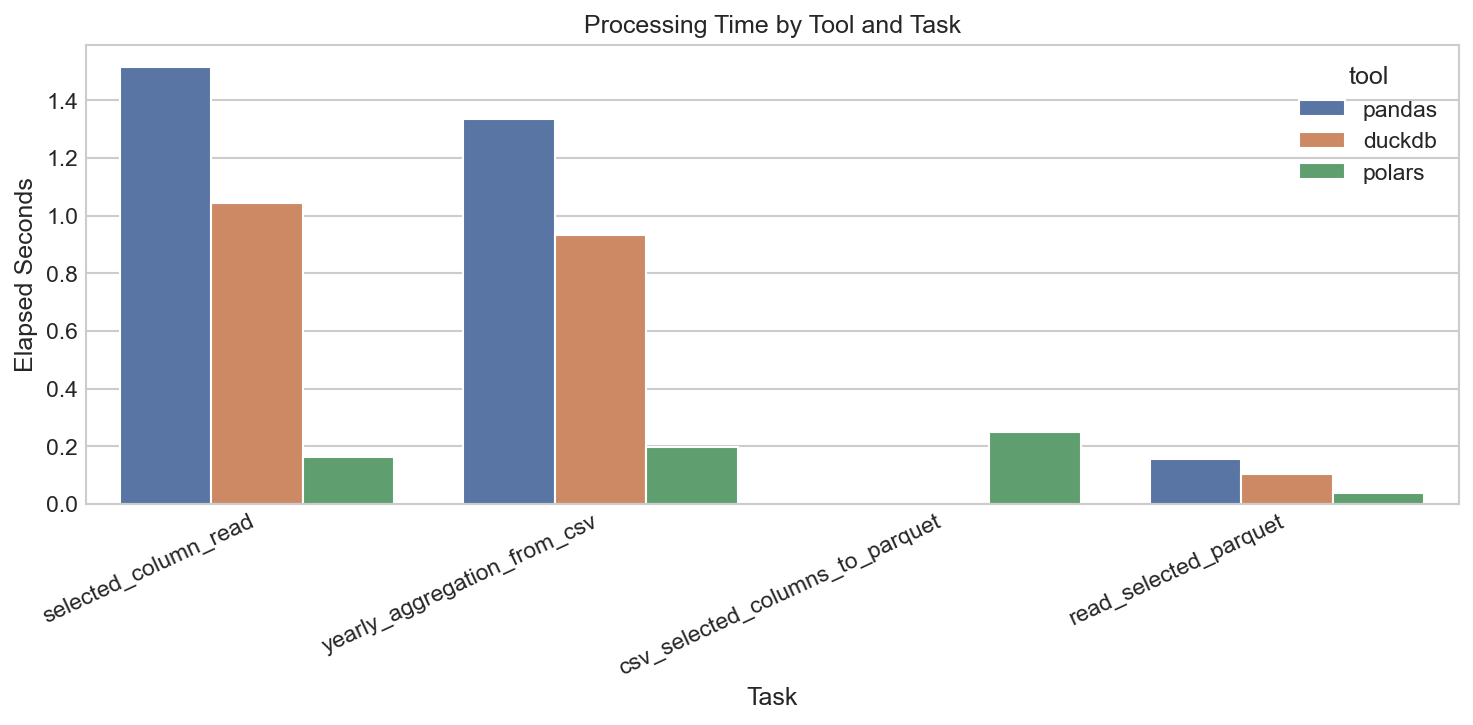
\includegraphics[width=0.9\textwidth]{../../figures/04_processing_time_by_tool_and_task.png}
  \caption{不同工具处理时间对比}
  \label{fig:tool-time}
\end{figure}

\section{数据清洗与特征工程}

\subsection{数据质量检查}
\placeholder{说明检查了缺失值、重复值、异常范围。特别说明 pct\_pos\_total 和 pct\_pos\_recent 中的 -1 是不可用值，不应该当作真实百分比。}

\subsection{基础预处理}
\placeholder{说明 release\_date 转换为日期，构造 release\_year；数值字段转换；多标签字段解析；保留原始字段并新增辅助字段。}

\subsection{特征工程}
\placeholder{列出主要特征：game\_age\_years、is\_free、platform\_count、review\_count\_calc、positive\_rate\_calc、genres\_count、tags\_count、description length、log 热度指标等。}

\section{Steam游戏市场结构分析}

\subsection{发行年份趋势}
\placeholder{根据 Notebook 04，用自己的话解释发行年份分布。可以写 2024 年是数据集中发行数量最高的年份，说明近年 Steam 游戏供给扩张明显。}

\begin{figure}[H]
  \centering
  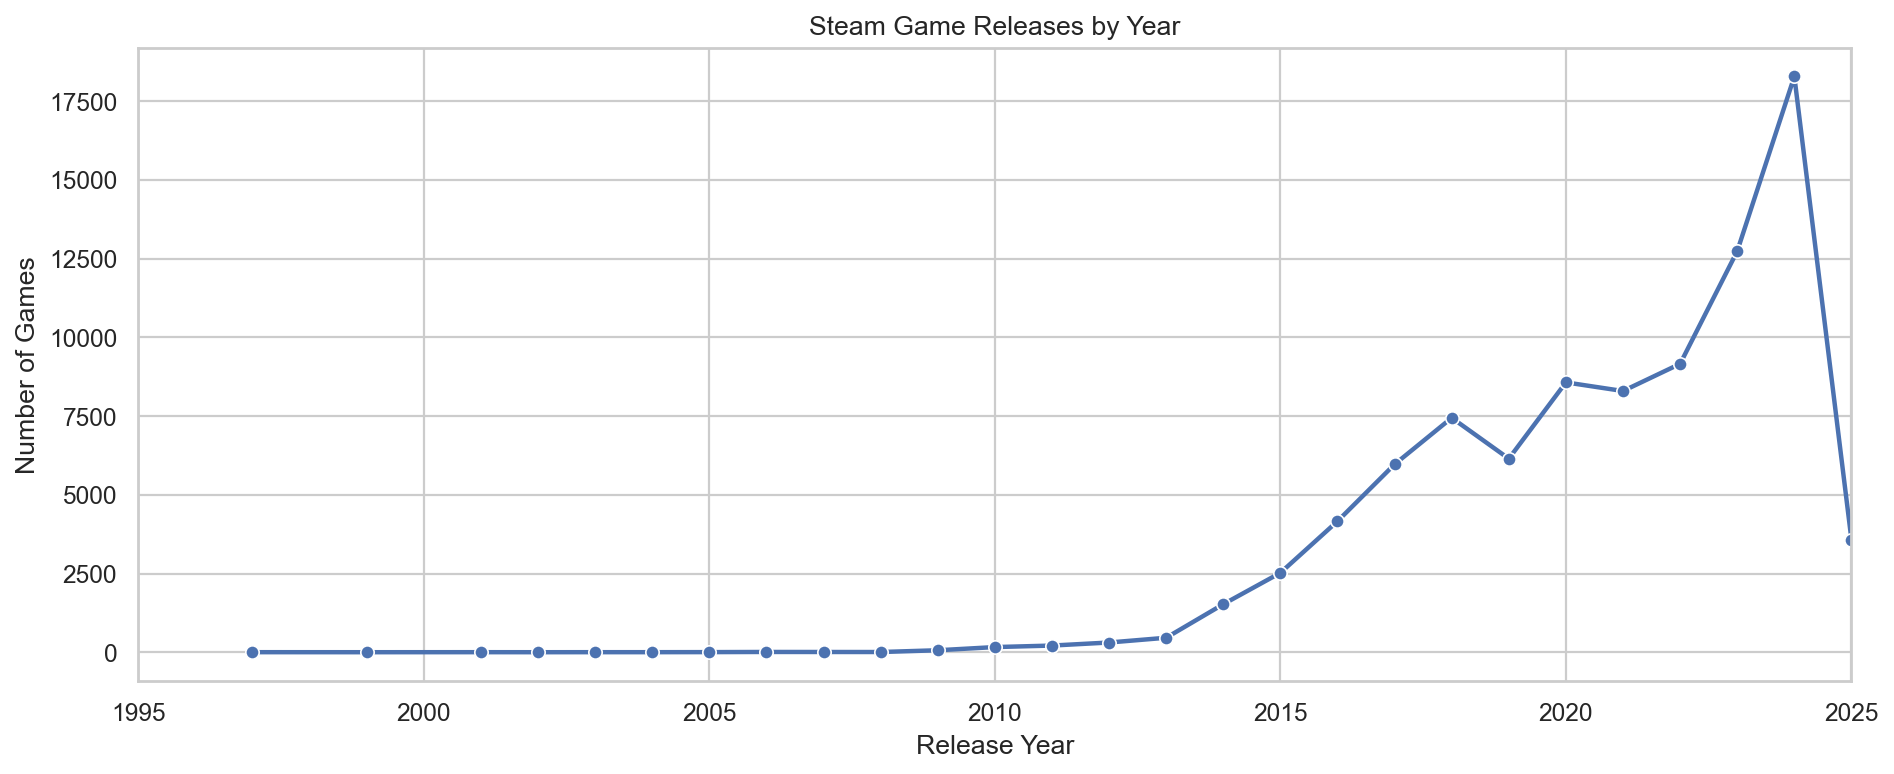
\includegraphics[width=0.88\textwidth]{../../figures/07_market_release_trend_by_year.png}
  \caption{Steam 游戏发行年份趋势}
  \label{fig:release-trend}
\end{figure}

\subsection{价格结构与免费游戏比例}
\placeholder{说明免费游戏约占 15.80\%，付费游戏仍占多数。可以讨论免费游戏降低进入门槛，但不能直接说明免费导致更高热度。}

\begin{figure}[H]
  \centering
  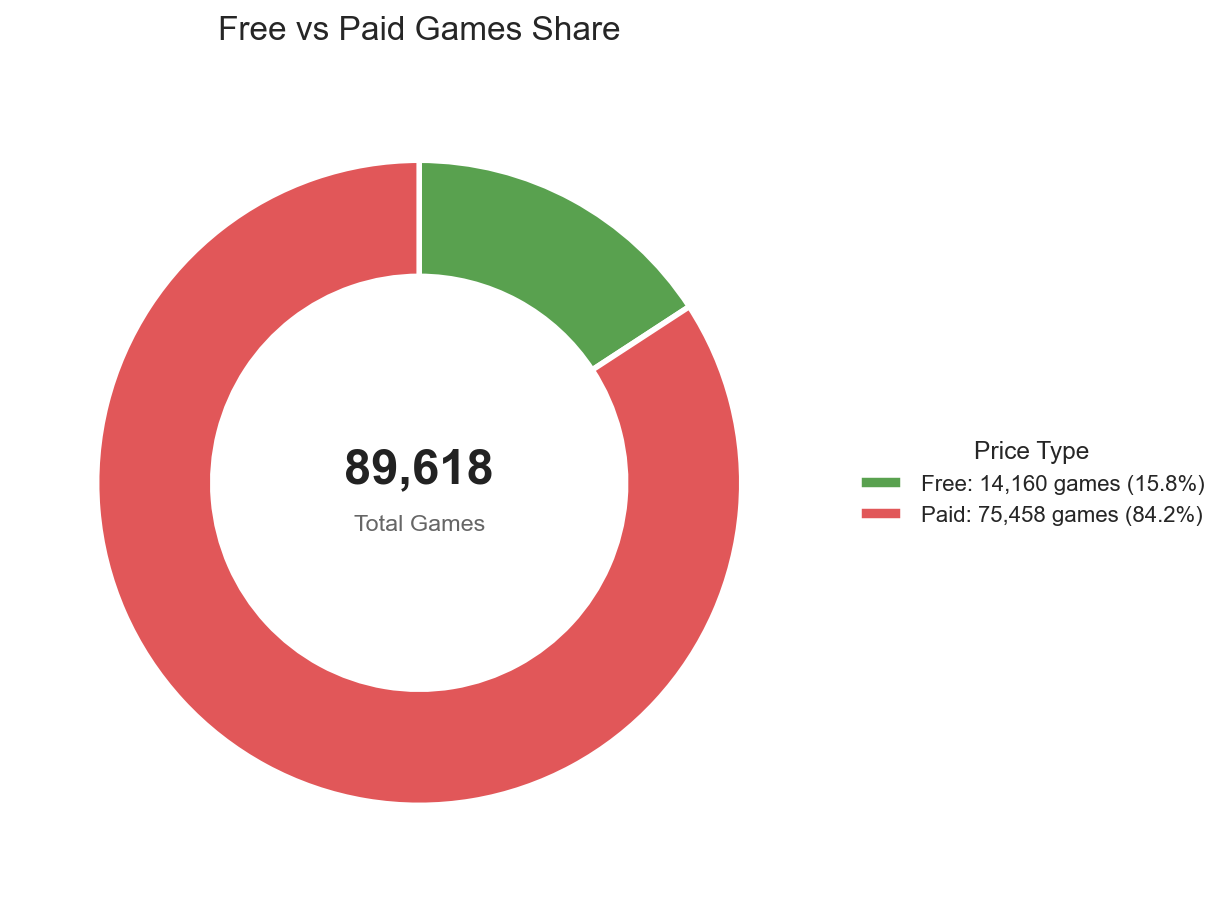
\includegraphics[width=0.72\textwidth]{../../figures/10_free_vs_paid_market_share.png}
  \caption{免费游戏与付费游戏占比}
  \label{fig:free-paid}
\end{figure}

\subsection{平台支持与开发者长尾}
\placeholder{说明 Windows 支持是基础结构，多平台游戏约占 23.05\%。同时开发商和发行商分布具有长尾特征，说明 Steam 市场由头部主体和大量中小主体共同构成。}

\section{玩家反馈与热度分析}

\subsection{评论数量的长尾分布}
\placeholder{写明评论数量高度长尾。当前数据中 72,563 款游戏至少有一条评论，33,358 款游戏达到 30 条及以上评论。评论数中位数为 13，均值约 1,479.70。}

\begin{figure}[H]
  \centering
  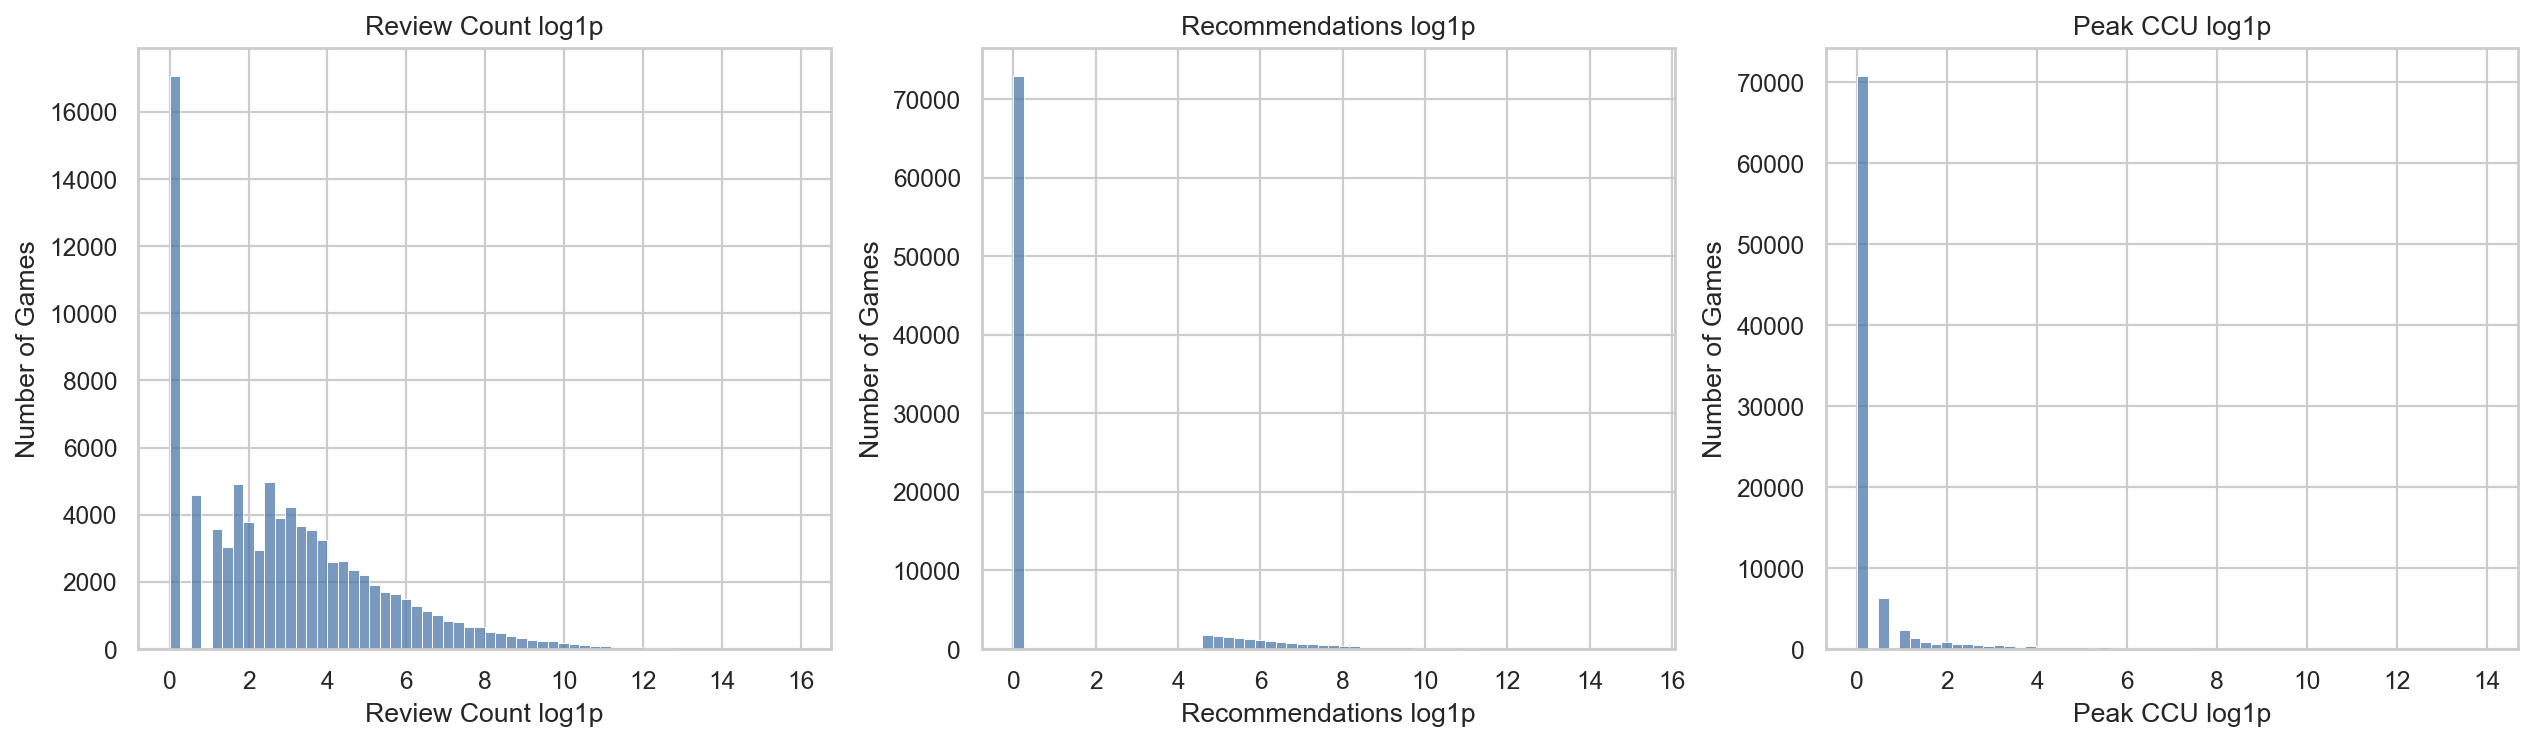
\includegraphics[width=0.95\textwidth]{../../figures/19_attention_metrics_log_distributions.png}
  \caption{玩家关注指标的 log 分布}
  \label{fig:attention-dist}
\end{figure}

\subsection{好评率与评论数量门槛}
\placeholder{说明好评率需要结合评论数理解。评论数很少时好评率不稳定，因此分析中使用 30 条评论作为较稳健门槛。}

\subsection{推荐数、峰值在线与游玩时长}
\placeholder{说明推荐数、峰值在线和游玩时长都是热度或参与度指标，但含义不同。总结它们与评论数之间的相关关系，但注意不要写成因果关系。}

\subsection{价格、平台与热度关系}
\placeholder{根据 Notebook 05 结果，讨论价格区间、免费/付费、多平台属性与热度指标的关系。强调这是描述性观察，不证明因果。}

\section{标签、类型与市场定位分析}

\subsection{标签体系的基本结构}
\placeholder{说明数据中解析出 33 个类型、40 个分类和 452 个标签，平均每款游戏约 11.26 个标签。标签比类型更细，更适合描述市场定位。}

\begin{figure}[H]
  \centering
  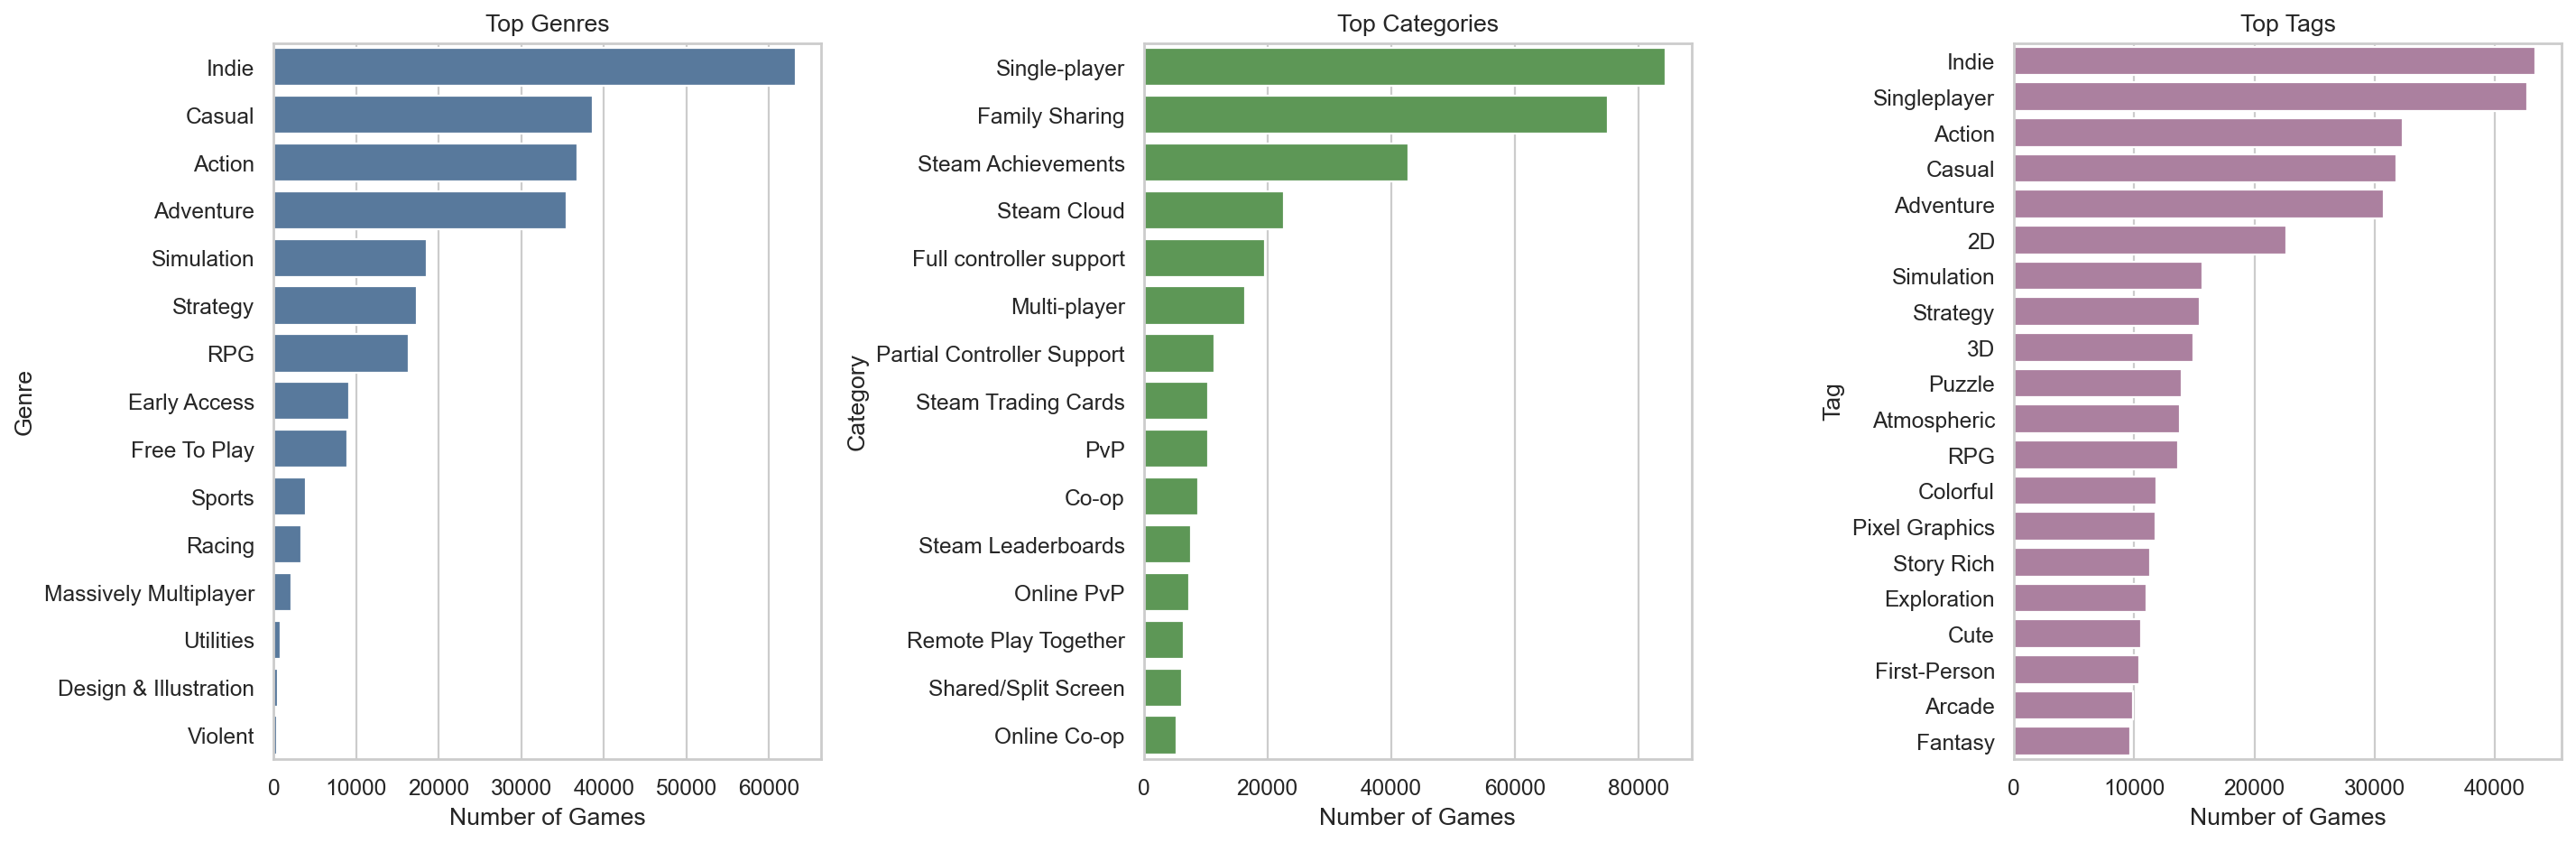
\includegraphics[width=0.95\textwidth]{../../figures/31_tag_genre_category_frequency.png}
  \caption{类型、分类与标签频次}
  \label{fig:tag-frequency}
\end{figure}

\subsection{标签竞争度与反馈表现}
\placeholder{解释横轴“标签覆盖游戏数量”可以作为竞争度代理，纵轴好评率反映反馈倾向。可以讨论高频标签不一定好评更高，低竞争高反馈标签值得进一步关注。}

\begin{figure}[H]
  \centering
  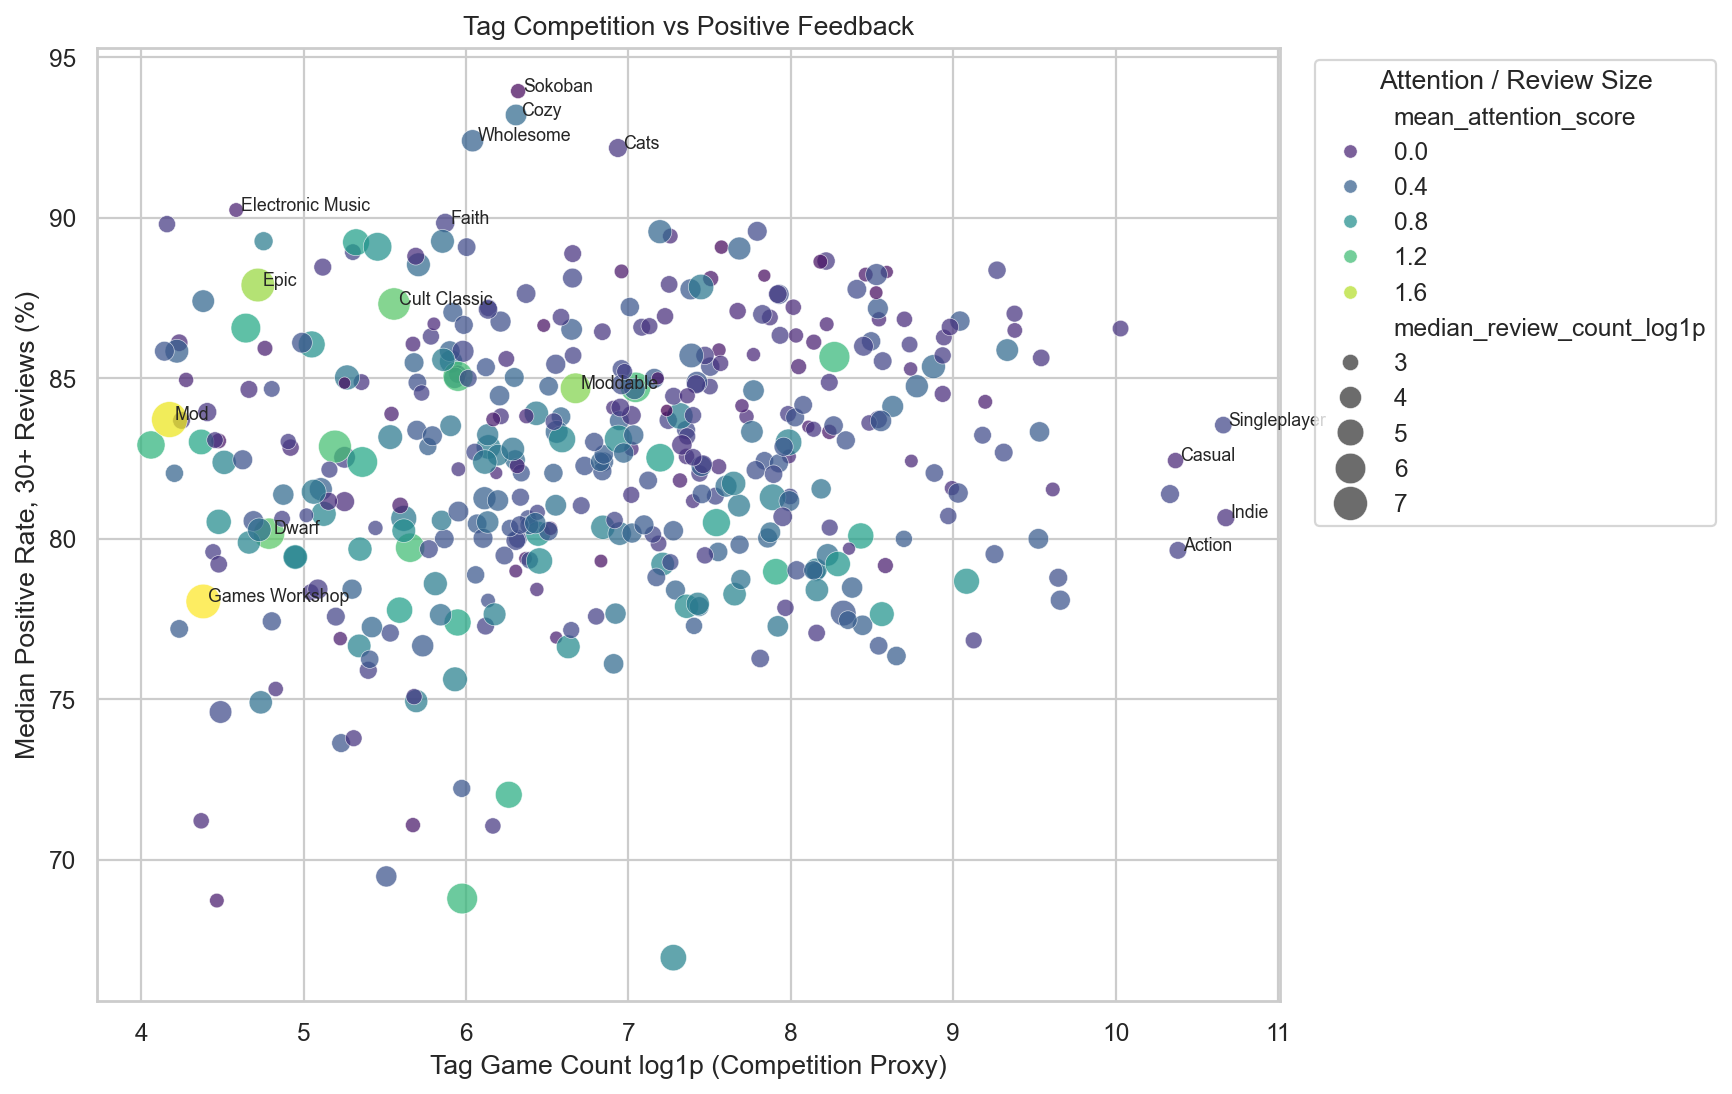
\includegraphics[width=0.88\textwidth]{../../figures/32_tag_competition_vs_positive_feedback.png}
  \caption{标签竞争度与好评率}
  \label{fig:tag-competition}
\end{figure}

\subsection{标签共现与类型定位}
\placeholder{说明标签经常组合出现，例如 Indie + Singleplayer 是较强共现组合之一。genre-tag 矩阵可以帮助理解粗类型和细标签之间的关系。}

\subsection{独立游戏子市场}
\placeholder{说明 Indie 是最常见的市场定位之一，但 Indie 内部还可以继续拆分。Notebook 06 中 Short 在 Indie 定位游戏中相对更突出。}

\section{综合结论}

\subsection{对研究问题的回答}
\placeholder{用你自己的话回答两个核心研究问题。建议分两段：第一段回答“哪些游戏更容易获得关注”；第二段回答“2024 到 2025 的变化”。这里是报告最核心部分，请尽量自己写。}

\subsection{主要发现}
\placeholder{用 3--5 条总结最重要发现。建议覆盖：市场扩张、长尾结构、评论/热度长尾、标签定位价值、快照变化。}

\subsection{管理或实践启示}
\placeholder{如果想让报告更像“分析报告”，可以写一点实践启示：例如开发者需要关注定位差异，不能只追逐高频标签；分析平台数据时要注意头部游戏对平均值的影响。}

\section{不足与改进方向}

\subsection{当前不足}
\placeholder{说明数据来自第三方 Kaggle；分析以描述性为主；不能证明因果；快照口径可能变化；标签不完全等于真实内容；大型数据文件不提交但可再生成。}

\subsection{后续方向}
\placeholder{说明后续可做 PCA、聚类、简单评分预测或相似游戏推荐系统。推荐系统可以使用 tags、genres、categories 和文本描述计算相似度，再用评论数、好评率、热度指标进行过滤或排序。}

\section*{参考资料}
\addcontentsline{toc}{section}{参考资料}

\begingroup
\raggedright
\begin{enumerate}[label={[\arabic*]},itemsep=0.35em]
  \item Kaggle. Steam Games Dataset 2025. \url{https://www.kaggle.com/datasets/artermiloff/steam-games-dataset}
  \item Predicting the Popularity of Games on Steam. 项目参考论文，见 reports/references/。
  \item Data-Driven Classifications of Video Game Vocabulary. 项目参考论文，见 reports/references/。
  \item Enhancing Game Review Sentiment Classification on Steam Platform with Attention-Based BiLSTM. 项目参考论文，见 reports/references/。
  \item Category-based and Popularity-guided Video Game Recommendation / CPGRec+. 项目参考论文，见 reports/references/。
\end{enumerate}
\par
\endgroup

\end{document}
